\section{Itération2: nouveau BS englobant TCP serveur}
    \subsection{Conception}
    Cette partie repose sur la modification des exigences et la nouvelle Conception
        \subsubsection{L'évolution des exigences}
            Après avoir fait l’évaluation des résultats de performance 
            de la 1ere itération du projet, on a redéfinit les spécifications du projet. 
            Le tableau suivant montre la différence des exigences entre les deux itérations:
            \\
            \begin{table}[h!]
            \centering
            \begin{tabular}{|p{3cm}|p{3cm}|p{4cm}|p{5cm}|}
                \hline
                \multicolumn{4}{|c|}{Les changements des exigences } \\
                \hline   & Itération1 & Itération2 & Avantage de cette évolution\\
                \hline
                Protocol de communication & MQTT & TCP avec le support de MQTT &
                Moins coûteux par rapport aux paquets échangés, tout en gardant 
                la possibilité de connecter le boîtier à un serveur MQTT \\
                \hline
                Architecture du BS  &  Un cluster de brokers MQTT avec des 
                subscribers des tracks et publishers d’events.  & Un cluster de 
                TCP serveur qui gèrent les connexions, traitent les message échangés 
                et envoient/re\c coivent les msg à/de kafka. & Moins coûteux par 
                rapport aux instances à gérer. 
                Plus facile à gérer un seul composant au BS. 
                Pas de complexité à dispatcher les subscribers quand on monte de charge.\\
                \hline 
            \end{tabular}
            \caption{Tableau de comparaison des exigences du projet}
            \label{table:1}
        \end{table} \\
    
        L’une des majeurs modifications est d'abandonner l’intégration du standard MQTT 
        tel qu il est . On ne garde que le Header de MQTT comme le Header des messages 
        échangés avec le nouveau tcp serveur. Ceci a pour but de garder la compatibilité 
        avec MQTT pour satisfaire les besoins commerciaux. 

        \subsubsection{Architecture de l'itération 2 }
            L’architecture du nouveau BS est conçue d’une façon à ce qu il présente 
            une solution aux problèmes rencontrés par l’architecture de la 1ere itération. 
            La figure ci dessous montre les composants de la nouvelle architecture:  \\
            \begin{figure}[ht]
                \centering
                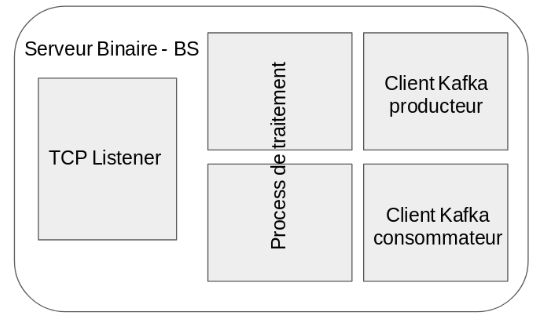
\includegraphics[scale=0.8]{\images/architecture_BS_iteration2.png}
                \caption{La conception de l'architecture du BS de l'itération 2}
                \label{Figure }
            \end{figure}
        
       
            Le BS  repose sur 3 grands composants: 
            En premier temps, le TCP serveur qui gère la connexion avec le boitier. 
            En deuxième temps,le traitement des données doit être gérer en parallèle. 
            Ce traitement assure l’encodage du protobuf boitier au protobuf cloud et 
            vis-versa. 
            D’autre part, deux clients kafka, un producteur qui va publier les messages 
            encodés et un autre consommateur qui va recevoir les messages d event. 

            \subsection{Implémentation}
            Le nouveau BS lance les diverses traitements dans des traitements en 
            parallèle. L’implémentation de ces processus parallèles s’effectuent grâce 
            aux goroutines du langage go, ce qui englobe toutes les fonctionnalités du BS 
            dans un même composant unifié.

            \subsubsection{Control plane}
             Concernant le flux de données ou Control plane, la communication entre 
             ces processus se fait comme le présente la figure ci-dessous: \\

             \begin{figure}[ht]
                \centering
                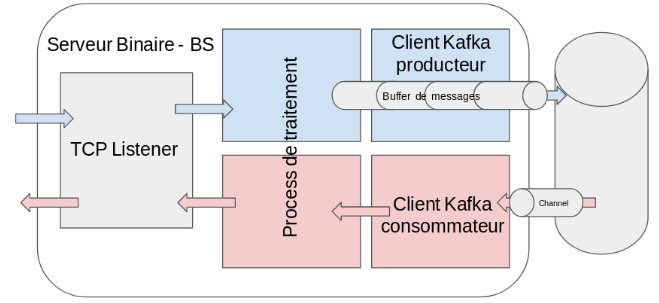
\includegraphics[scale=0.8]{\images/control_plane.png}
                \caption{Le flux de données du BS de l'itération 2}
                \label{Figure }
            \end{figure}


            * Le boitier envoie un track pour le cloud: 


            La première connexion se fait avec le TCP Listener. 
            Comme son nom l’indique, ce composant écoute, vérifie et  maintient la 
            connexion avec les boîtiers. Il est considéré comme le Générateur. 
            Après avoir vérifier la connexion avec un boitier donné, il envoie le 
            message reçu au processus de traitement dans un channel. \\
            Ce dernier décode le format du message et l’encode en format des données du 
            cloud. Ensuite il le met dans un buffer des messages prêts à la publication 
            kafka. Puis le client kafka envoie tous les messages du buffer d’une manière 
            périodique de quelques secondes.\\ 
            L’envoi des messages d’une manière périodique minimise l'accès 
            écriture dans la BD ce qui augmente l’efficacité du traitement global. 

            *  Le cloud envoie un event au boîtier: 
            Le service qui a déclenché l’event va publier dans le broker des messages le 
            message dans un topic spécifique. Le client consommateur est toujours en écoute sur ce topic, 
            il reçoit le message et l'envoie directement au traitement. Le message s’encode avec le format 
            protobuf du boitier est maintenant prêt à être envoyer au boîtier. Le TCP listener s’occupe alors 
            de son envoi à son boitier. \\
            Il est à noter que l'implémentation de cet envoi par rapport à plusieurs 
            instances sera plus complexe. 

        
        \begin{itemize}
            \renewcommand{\labelitemi}{$\bullet$}
            \item \textbf{Explicit Mutability}: Une variable est, par défaut,
            immuable (invariable ? :)). Pour la faire varier le code doit la
            déclarer explicitement mutable, avec le mot clé \textit{mut}.
            \begin{lstlisting}[autogobble, language=Rust, style=boxed]
                let a = 5;
                a = 3; // Error, a not mutable
                let mut a = 5;
                a = 3; // OK
            \end{lstlisting}

            \item \textbf{Ownership}: C'est un système de manipulation des données basé
            sur le fait que chaque donnée a un propriétaire. Elle ne peut pas avoir
            plusieurs propriétaires; par contre elle peut changer de propriétaire,
            être consommée en quelque sorte; cette opération s'appelle un move.
            Elle est effectuée sur les types qui n'implémentent pas le trait Copy.
            \begin{lstlisting}[autogobble, language=Rust, style=boxed]
                let a = SomeStruct::new();
                let b = a;
                a.use(); // Error, use after move
            \end{lstlisting}

            \item \textbf{Borrowing}: Une valeur \textit{owned} par une certaine variable
            peut être "prêtée", par réference. Cela s'appelle le borrowing
            et a des règles très strictes, enforcées par le \textbf{BorrowChecker}.
            Une variable peut avoir une réference mutable ou plusieurs réferences
            non-mutables.
            \begin{lstlisting}[autogobble, language=Rust, style=boxed]
                let a = SomeStruct::new();
                let b = &a; // Ok
                let mut c = &a; // Ok, the borrow itself is not mutable
                let d = &mut a; // Error, immutable borrow still in context
            \end{lstlisting}
        \end{itemize}
        \bigskip
        Le but de cette explication est de montrer la différence considérable
        avec d'autres langages de programmation. Un lecteur intéressé pourra
        apprendre le langage pour plus d'informations.

    \subsection{Implémentation}
        \subsubsection{Go un language pas POO}
        Les bugs dans le code arrivent même avec les programmeurs les plus aptes.
        \company{} ne fait pas exception à cette règle. Dans l'effort de minimiser
        ces bugs le plus possible, \gls{mdi} a fait le choix de migrer vers Rust.
        Trois nouveaux projets sont développés en Rust:
        \begin{itemize}
            \renewcommand{\labelitemi}{$\bullet$}
            \item MD30, Un nouveau protocol de communication dongle-cloud
            \item MEP, Morpheus event processor, un outil de programmation graphique
            \item MSP, Morpheus signal processor, un moteur de traitement de signaux
        \end{itemize}
        \bigskip
        Go présente un grand nombre d'avantages, mais aussi un grand nombre
        d'inconvénients. Pour une personne qui fait de la programmation orientée
        objets, s'adapter n'est pas trivial. Mais une fois on s'habitue aux
        dynamiques de ce languages, on retrouve qu'il est assez flexible.\\[0.3cm]
        Par contre, il faut s'attendre à se heurter à des bugs, de.... 
        De même il faut être prêt à implémenter des bibliothèques rudimentales,..\\[0.3cm]
        Ci-dessous un bilan des principaux avantages et inconvénients de Rust par
        rapport à autres languages, notament C++.

        \subsubsection{Avantages}
            \begin{itemize}
                \renewcommand{\labelitemi}{$\bullet$}
                \item Garanties thread-safety
                \item "Si \c ca compile, \c ca marche"
                \item Communauté active
                \item Bonne gestions de cas, pas de comportement indéterminé
                \item Performances très bonnes
                \item Gestion facile de bibliothèques (Cargo)
                \item Cross-compilation facile (Cargo)
                \item Evolution du language
            \end{itemize}

        \subsubsection{Inconvénients}
            \begin{itemize}
                \renewcommand{\labelitemi}{$\bullet$}
                \item Instabilités compilateur, parfois dans la chaine stable
                \item Manque d'expertises Rust en entreprise
                \item Known issues sans perspectives de fixes
                \item Manque d'optimisations spécifiques aux processeurs
                \item Complexité de codes simples dans autres languages
                \item Pas de programmation orientée objets
                \item Dynamic dispatch très limité
                \item Chaine de compilation non-optimale pour notre processeur
                \item Communauté très jeune
                \item Bibliothèques essentielles absentes
            \end{itemize}

    \subsection{Test }
        Apprendre Rust était une très belle expérience. La réference principale
        pour moi était le Rust book\cite{rust_book}. J'ai lu ce livre entier,
        et suivi les examples. Il couvre assez succintement les détails du
        language.\\[0.3cm]
        Le Rustonomicon\cite{rust_unsafe_book} m'a servi de réference pour
        comprendre des concepts sur le fonctionnement interne du language.
        \'Evidemment, pour profiter de Rust il m'a fallu éviter, le plus possible,
        les syntaxes \textbf{unsafe}. En effet, je n'en ai eu besoin que pour les
        s, et l'intégration avec .. Mais ce livre m'a aidé à
        comprendre un certain nombre de problèmes auquels j'ai fait face, notament:
        \begin{itemize}
            \renewcommand{\labelitemi}{$\bullet$}
            \item La notion de variance de structures\cite{variance_wiki}.
            \item Les erreurs de lifetimes
            \item Coercions de types
            \item Le unwind de threads
            \item Les phantom data
            \item Drop et l'utilisation de \textbf{Option} dans des cas spéciaux
        \end{itemize}
        \bigskip
        Il faut aussi dire que le bagage fourni par le cours de compilation à
        \establishment{} était d'une utilité exceptionnelle, surtout que
        programmer en Rust, c'est virtuellement une conversation avec le
        compilateur!\\[0.3cm]
        Mais la piste principale pour l'apprentissage reste la pratique. Et avec
        le projet \gls{msp} j'ai eu la chance de faire des fautes, réitérer,
        apprendre des concepts et des patterns, et corriger, dans un cycle qui a
        duré 4 mois. Les détails du code seront discutés dans la section
        concernant ce projet.

    \subsection{Amélioration à effectuer}
        Data plane .. 
        Rust étant un langage très jeune, j'ai saisi l'opportunité pour contribuer
        à son développement, que ce soit en discutant avec la communauté, et en
        proposant des idées dans les issues (sur github), ou en publiant des crates sur
        crates.io\cite{crates_io}. Malgré mon désir de le faire, je n'ai pas eu
        le temps, jusqu'aujourd'hui, de contribuer au projet du language même.\\[0.3cm]
        Durant le projet \gls{msp}, j'ai publié le crate
        "ts-mem-pool"\cite{mem_pool}, développé dans le cadre de ce projet.
        C'est une simple implémentation de memory pool léger, générique et avec
        des élements thread-safe. J'ai aussi écrit, avec un collègue, un binding
        en Rust pour la bibliothèque iir1\cite{iir1}, qui attend encore sa publication.
